%beamer

% TODO: Jede menge:
% Reguläre Ausdrüke in \rx umwandeln
% * Problem mit \rx fixen
% Folien ab "Zusammenhang..." besser einarbeiten
% Besser auf Zusammenhänge eingehen
% Besserer Aufbau der Beispiele und Aufgaben
% Strukturelle Induktion: Bessere Einführung, neues Beispiel, neue Aufgabe

% Define a global usable date. Must come before StyleTut
%\newcommand{\mydate}{03.02.2017}

% Comment/uncomment this line to toggle handout mode
%\newcommand{\handout}{}

% % \bigtimes abgeschrieben von http://tex.stackexchange.com/questions/14386/importing-a-single-symbol-from-a-different-font
% \DeclareFontFamily{U}{mathx}{\hyphenchar\font45}
% \DeclareFontShape{U}{mathx}{m}{n}{
%       <5> <6> <7> <8> <9> <10> gen * mathx
%       <10.95> mathx10 <12> <14.4> <17.28> <20.74> <24.88> mathx12
%       }{}
% \DeclareSymbolFont{mathx}{U}{mathx}{m}{n}
% \DeclareMathSymbol{\bigtimes}{\mathop}{mathx}{161}

\RequirePackage{xcolor}

\def\9{\square}
%\def\9{\blank}

% f"ur Aussagenlogik
\colorlet{alcolor}{blue}
\RequirePackage{tikz}
\usetikzlibrary{arrows.meta}
\newcommand{\alimpl}{\mathrel{\tikz[x={(0.1ex,0ex)},y={(0ex,0.1ex)},>={Classical TikZ Rightarrow[]}]{\draw[alcolor,->,line width=0.7pt,line cap=round] (0,0) -- (15,0);\path (0,-6);}}}
\newcommand{\aleqv}{\mathrel{\tikz[x={(0.1ex,0ex)},y={(0ex,0.1ex)},>={Classical TikZ Rightarrow[]}]{\draw[alcolor,<->,line width=0.7pt,line cap=round] (0,0) -- (18,0);\path (0,-6);}}}
\newcommand{\aland}{\mathbin{\raisebox{-0.6pt}{\rotatebox{90}{\texttt{\color{alcolor}\char62}}}}}
\newcommand{\alor}{\mathbin{\raisebox{-0.8pt}{\rotatebox{90}{\texttt{\color{alcolor}\char60}}}}}
%\newcommand{\ali}[1]{_{\mathtt{\color{alcolor}#1}}}
\newcommand{\alv}[1]{\mathtt{\color{alcolor}#1}}
\newcommand{\alnot}{\mathop{\tikz[x={(0.1ex,0ex)},y={(0ex,0.1ex)}]{\draw[alcolor,line width=0.7pt,line cap=round,line join=round] (0,0) -- (10,0) -- (10,-4);\path (0,-8) ;}}}
\newcommand{\alP}{\alv{P}} %ali{#1}}
%\newcommand{\alka}{\negthinspace\hbox{\texttt{\color{alcolor}(}}}
\newcommand{\alka}{\negthinspace\text{\texttt{\color{alcolor}(}}}
%\newcommand{\alkz}{\texttt{\color{alcolor})}}\negthinspace}
\newcommand{\alkz}{\text{\texttt{\color{alcolor})}}\negthinspace}
\newcommand{\AAL}{A_{AL}}
\newcommand{\LAL}{\hbox{\textit{For}}_{AL}}
\newcommand{\AxAL}{\hbox{\textit{Ax}}_{AL}}
\newcommand{\AxEq}{\hbox{\textit{Ax}}_{Eq}}
\newcommand{\AxPL}{\hbox{\textit{Ax}}_{PL}}
\newcommand{\AALV}{\hbox{\textit{Var}}_{AL}}
\newcommand{\MP}{\hbox{\textit{MP}}}
\newcommand{\GEN}{\hbox{\textit{GEN}}}
\newcommand{\W}{\ensuremath{\hbox{\textbf{w}}}\xspace}
\newcommand{\F}{\ensuremath{\hbox{\textbf{f}}}\xspace}
\newcommand{\WF}{\ensuremath{\{\W,\F\}}\xspace}
\newcommand{\val}{\hbox{\textit{val}}}
\newcommand{\valDIb}{\val_{D,I,\beta}}

\newcommand*{\from}{\colon}

% die nachfolgenden Sachen angepasst an cmtt
\newlength{\ttquantwd}
\setlength{\ttquantwd}{1ex}
\newlength{\ttquantht}
\setlength{\ttquantht}{6.75pt}
\def\plall{%
  \tikz[line width=0.67pt,line cap=round,line join=round,baseline=(B),alcolor] {
    \draw (-0.5\ttquantwd,\ttquantht) -- node[coordinate,pos=0.4] (lll){} (-0.25pt,-0.0pt) -- (0.25pt,-0.0pt) -- node[coordinate,pos=0.6] (rrr){} (0.5\ttquantwd,\ttquantht);
    \draw (lll) -- (rrr);
    \coordinate (B) at (0,-0.35pt);
  }%
}
\def\plexist{%
  \tikz[line width=0.67pt,line cap=round,line join=round,baseline=(B),alcolor] {
    \draw (-0.9\ttquantwd,\ttquantht) -- (0,\ttquantht) -- node[coordinate,pos=0.5] (mmm){} (0,0) --  (-0.9\ttquantwd,0);
    \draw (mmm) -- ++(-0.75\ttquantwd,0);
    \coordinate (B) at (0,-0.35pt);
  }\ensuremath{\,}%
}
\let\plexists=\plexist
\newcommand{\NT}[1]{\ensuremath{\langle\mathrm{#1} \rangle}}

\newcommand{\CPL}{\text{\itshape Const}_{PL}}
\newcommand{\FPL}{\text{\itshape Fun}_{PL}}
\newcommand{\RPL}{\text{\itshape Rel}_{PL}}
\newcommand{\VPL}{\text{\itshape Var}_{PL}}
\newcommand{\ATer}{A_{\text{\itshape Ter}}}
\newcommand{\ARel}{A_{\text{\itshape Rel}}}
\newcommand{\AFor}{A_{\text{\itshape For}}}
\newcommand{\LTer}{L_{\text{\itshape Ter}}}
\newcommand{\LRel}{L_{\text{\itshape Rel}}}
\newcommand{\LFor}{L_{\text{\itshape For}}}
\newcommand{\NTer}{N_{\text{\itshape Ter}}}
\newcommand{\NRel}{N_{\text{\itshape Rel}}}
\newcommand{\NFor}{N_{\text{\itshape For}}}
\newcommand{\PTer}{P_{\text{\itshape Ter}}}
\newcommand{\PRel}{P_{\text{\itshape Rel}}}
\newcommand{\PFor}{P_{\text{\itshape For}}}

\newcommand{\plka}{\alka}
\newcommand{\plkz}{\alkz}
%\newcommand{\plka}{\plfoo{(}}
%\newcommand{\plkz}{\plfoo{)}}
\newcommand{\plcomma}{\hbox{\texttt{\color{alcolor},}}}
\newcommand{\pleq}{{\color{alcolor}\,\dot=\,}}

% MODIFIED (DJ)
% previously: \newcommand{\plfoo}[1]{\mathtt{\color{alcolor}#1}}
\newcommand{\plfoo}[1]{\texttt{\color{alcolor}#1}}

\newcommand{\plc}{\plfoo{c}}
\newcommand{\pld}{\plfoo{d}}
\newcommand{\plf}{\plfoo{f}}
\newcommand{\plg}{\plfoo{g}}
\newcommand{\plh}{\plfoo{h}}
\newcommand{\plx}{\plfoo{x}}
\newcommand{\ply}{\plfoo{y}}
\newcommand{\plz}{\plfoo{z}}
\newcommand{\plR}{\plfoo{R}}
\newcommand{\plS}{\plfoo{S}}

\newcommand{\bv}{\mathrm{bv}}
\newcommand{\fv}{\mathrm{fv}}

%\newcommand{\AxAL}{\hbox{\textit{Ax}}_{AL}}
%\newcommand{\AALV}{\hbox{\textit{Var}}_{AL}}

%\renewcommand{\#}[1]{\literal{#1}}
\newcommand{\A}{\mathcal{A}}
\newcommand{\Adr}{\text{Adr}}
\newcommand{\ar}{\mathrm{ar}}
\newcommand{\ascii}[1]{\literal{\char#1}}
%\newcommand{\assert}[1]{\text{/\!\!/\ } #1}
\newcommand{\assert}[1]{\colorbox{black!7!white}{\ensuremath{\{\;#1\;\}}}}
\newcommand{\Assert}[1]{$\langle$\textit{#1}$\rangle$}
\newcommand{\B}{\mathcal{B}}
\newcommand{\bfmod}{\mathbin{\kw{ mod }}}
\newcommand{\bb}{{\text{bb}}}
\def\bottom{\hbox{\small$\pmb{\bot}$}}
\newcommand{\card}[1]{|#1|}
%\newcommand{\cod}{\mathop{\text{cod}}}  % ist in thwmathabbrevs
\newcommand{\Conf}{\mathcal{C}}
\newcommand{\define}[1]{\emph{#1}}
%\renewcommand{\dh}{d.\,h.\@\xspace}
%\newcommand{\Dh}{D.\,h.\@\xspace}
%\newcommand{\engl}[1]{engl.\xspace\emph{#1}}
\newcommand{\eps}{\varepsilon}
%\newcommand{\evtl}{evtl.\@\xspace}
\newcommand{\fbin}{\text{bin}}
\newcommand{\finv}{\text{inv}}
\newcommand{\fnum}{\text{num}}
\newcommand{\fNum}{{\text{Num}}}
\newcommand{\frepr}{\text{repr}}
\newcommand{\fRepr}{\text{Repr}}
\newcommand{\fZkpl}{\text{Zkpl}}
\newcommand{\fLen}{\text{Len}}
\newcommand{\fsem}{\text{sem}}
\providecommand{\fspace}{\mathord{\text{space}}}
\providecommand{\fSpace}{\mathord{\text{Space}}}
\providecommand{\ftime}{\mathord{\text{time}}}
\providecommand{\fTime}{\mathord{\text{Time}}}
\newcommand{\fTrans}{\text{Trans}}
\newcommand{\fVal}{\text{Val}}

% MODIFIED (DJ)
\newcommand{\Val}{\text{Val}}

%\def\G{\mathbb{Z}}
\newcommand{\HT}[1]{\normalfont\textsc{HT-#1}}
\newcommand{\htr}[3]{\{#1\}\;#2\; \{#3\}}
\newcommand{\Id}{\text{I}}
%\newcommand{\ie}{i.\,e.\@\xspace}
\newcommand{\instr}[2]{\texttt{#1}\ \textit{#2}}
\newcommand{\Instr}[2]{\texttt{#1}\ \textrm{#2}}
\newcommand{\instrr}[3]{\texttt{#1}\ \textit{#2}\texttt{(#3)}}
\newcommand{\Instrr}[3]{\texttt{#1}\ \textrm{#2}\texttt{(#3)}}
\newcommand{\io}{\!\mid\!}
\usepackage{KITcolors}
\newcommand{\literal}[1]{\hbox{\textcolor{blue!95!white}{\textup{\texttt{\scalebox{1.11}{#1}}}}}}
%\newcommand{\literal}[1]{\hbox{\textcolor{KITblue!80!black}{\textup{\texttt{#1}}}}}
\def\kasten#1{\leavevmode\literal{\setlength{\fboxsep}{1pt}\fbox{\vrule  width 0pt height 1.5ex depth 0.5ex #1}}}
\newcommand{\kw}[1]{\ensuremath{\mathbf{#1}}}
\newcommand{\lang}[1]{\ensuremath{\langle#1\rangle}}
%\newcommand{\maw}{m.\,a.\,w.\@\xspace}
%\newcommand{\MaW}{M.\,a.\,w.\@\xspace}
\newcommand{\mdefine}[2][FOOBAR]{\define{#2}\def\foobar{FOOBAR}\def\optarg{#1}\ifx\foobar\optarg\def\optarg{#2}\fi\graffito{\optarg}}
\newcommand{\meins}{\rotatebox[origin=c]{180}{1}}
\newcommand{\Mem}{\text{Mem}}
\newcommand{\memread}{\text{memread}}
\newcommand{\memwrite}{\text{memwrite}}
\providecommand{\meta}[1]{\ensuremath{\langle}\textit{#1}\ensuremath{\rangle}}
%\newcommand{\N}{\mathbb{N}}
\newcommand{\NP}{\mathbf{NP}}
\newcommand{\Nadd}{N_{\text{add}}}
\newcommand{\Nmult}{N_{\text{mult}}}
% MODIFIED (DJ): added \!, mathcal{O}
\newcommand{\Oh}[1]{\mathcal{O}\!\left(#1\right)}
\newcommand{\Om}[1]{\Omega\!\left(#1\right)}
\newcommand{\personname}[1]{\textsc{#1}}
\newcommand{\regname}[1]{\texttt{#1}}
\newcommand{\mima}{\textsc{Mima}\xspace}
\newcommand{\mimax}{\textsc{Mima-X}\xspace}

\def\Pclass{\text{\bfseries P}}
\def\PSPACE{\text{\bfseries PSPACE}}

\newcommand{\SPush}{\text{push}}
\newcommand{\SPop}{\text{pop}}
\newcommand{\SPeek}{\text{peek}}
\newcommand{\STop}{\text{top}}
\newcommand{\STos}{\text{\itshape tos}}
\newcommand{\SBos}{\text{\itshape bos}}

%\newcommand{\R}{\mathbb{R}}
\newcommand{\Rnullplus}{\R_0^{+}}
\newcommand{\Rplus}{\R_{+}}
\newcommand{\resp}{resp.\@\xspace}
\newcommand{\Sem}{\text{Sem}}
\newcommand{\sgn}{\mathop{\text{sgn}}}
\newcommand{\sqbox}{\mathop{\raisebox{-6.2pt}{\hbox{\hbox to 0pt{$^{^{\sqcap}}$\hss}$^{^{\sqcup}}$}}}}
\newcommand{\sqleq}{\sqsubseteq}
\newcommand{\sqgeq}{\sqsupseteq}
% MODIFIED (DJ): added \!
\newcommand{\Th}[1]{\Theta\!\left(#1\right)}
%\newcommand{\usw}{usw.\@\xspace}
\newcommand{\V}[1]{\hbox{\textit{#1}}}
\newcommand{\x}{\times}
\newcommand{\ZK}{\mathbb{K}}
%\newcommand{\Z}{\mathbb{Z}}
\newcommand{\zB}{z.\,B.\@\xspace}
\newcommand{\ZB}{Z.\,B.\@\xspace}
% \newcommand{\bb}{{\text{bb}}}
% \def\##1{\hbox{\textcolor{darkblue}{\texttt{#1}}}}
% \def\A{\mathcal{A}}
% \newcommand{\0}{\#0}
% \newcommand{\1}{\#1}
% \newcommand{\Obj}{\text{Obj}}
% \newcommand{\start}{\mathop{\text{start}}}
% \newcommand{\compactlist}{\addtolength{\itemsep}{-\parskip}}
% \newcommand{\fval}{\text{val}}
% \newcommand{\lang}[1]{\ensuremath{\langle#1\rangle}}
% \newcommand{\io}{\!\mid\!}
% \def\sqbox{\mathop{\raisebox{-6.2pt}{\hbox{\hbox to 0pt{$^{^{\sqcap}}$\hss}$^{^{\sqcup}}$}}}}
% \def\sqleq{\sqsubseteq}
% \def\sqgeq{\sqsupseteq}
\def\Td{T_{\overline{d}}}
% \newcommand{\csym}[1]{\ensuremath{\#{c}_{\#{\hbox{\scriptsize #1}}}}}
% \newcommand{\F}{\ensuremath{\mathcal{F}}}
% \newcommand{\fsym}[2]{\ensuremath{\#{f}^{\#{\hbox{\scriptsize #1}}}_{\#{\hbox{\scriptsize #2}}}}}
% \newcommand{\rsym}[2]{\ensuremath{\#{R}^{\#{\hbox{\scriptsize #1}}}_{\#{\hbox{\scriptsize #2}}}}}
% \newcommand{\xsym}[1]{\ensuremath{\#{x}_{\#{\hbox{\scriptsize #1}}}}}
% \newcommand{\I}{\mathcal{I}}
% ********************************************************************

\usepackage{../TutTexbib/thwregex}

\newcommand{\nM}{\mathbb{M}}
\newcommand{\nR}{\mathbb{R}}
\newcommand{\nN}{\mathbb{N}}
\newcommand{\nZ}{\mathbb{Z}}
\newcommand{\nQ}{\mathbb{Q}}
\newcommand{\nB}{\mathbb{B}}
\newcommand{\nC}{\mathbb{C}}
\newcommand{\nK}{\mathbb{K}}
\newcommand{\nF}{\mathbb{F}}
\newcommand{\nG}{\mathbb{G}}
\newcommand{\nullel}{\mathcal{O}}
\newcommand{\einsel}{\mathds{1}}
\newcommand{\nP}{\mathbb{P}}
\newcommand{\Pot}{\mathcal{P}}
\renewcommand{\O}{\text{O}}

%\newcommand{\literal}[1]{\textcolor{blue}{\texttt{#1}}}
\newcommand{\realTilde}{\textasciitilde \ }
\newcommand{\setsize}[1]{\; \mid #1 \mid \; }

\definecolor{myRed}{RGB}{255,75,20}
\colorlet{myGreen}{KITpalegreen}

\newcounter{tfqtempcount}
\newcommand{\truefalseQ}[4]{
	\setcounter{tfqtempcount}{#1}
	\addtocounter{tfqtempcount}{1}
	\truefalseQuestion{#1}{\value{tfqtempcount}}{#2}{#3}{#4}
}
\newcommand{\truefalseQuestion}[5]{\item<#1-|handout:#1-> \color<#2-|handout:#2->{#3} #4 \qquad \visible<#2-|handout:#2->{#5}}

\newcommand{\boder}{\ensuremath{\textcolor{blue}{\vee}}\text{} }
\newcommand{\bund}{\ensuremath{\textcolor{blue}{\wedge}}\text{}}
\newcommand{\bimp}{\ensuremath{\textcolor{blue}{\to}}\text{}}
\newcommand{\bnot}{\ensuremath{\textcolor{blue}{\neg}}\text{}}
\newcommand{\bone}{\ensuremath{\textcolor{blue}{1}}\text{}}
\newcommand{\bzero}{\ensuremath{\textcolor{blue}{0}}\text{}}
\newcommand{\bleftBr}{\ensuremath{\textcolor{blue}{(}}\text{}}
\newcommand{\brightBr}{\ensuremath{\textcolor{blue}{)}}\text{}}

\newcommand{\summe}[2]{\sum\limits_{#1}^{#2}}
\newcommand{\limes}[1]{\lim\limits_{#1}}

\newcommand{\numpp}{\advance \value{weeknum} by -2 \theweeknum \advance \value{weeknum} by 2}
\newcommand{\nump}{\advance \value{weeknum} by -1 \theweeknum \advance \value{weeknum} by 1}

\newcommand{\mycomment}[1]{}

\newcounter{abc}
\newenvironment{alist}{
  \begin{list}{(\alph{abc})}{
      \usecounter{abc}\setlength{\leftmargin}{8mm}\setlength{\labelsep}{2mm}
    }
}{\end{list}}

\renewcommand{\mod}{\text{ \bf{mod} }}
\renewcommand{\div}{\text{ \bf{div} }}

%\newcommand{\sgn}{\text{sgn}}

% Toggle Handout mode by including this line before including style_tut:
% \newcommand{\handout}{}

%% Beamer-Klasse im korrekten Modus
\ifdefined \handout
\documentclass[handout]{beamer} % Handout mode
\else
\documentclass{beamer}
\fi


% Das ist der KIT-Stil
%\usepackage{../TutTexbib/beamerthemekit}
\usepackage[deutsch,titlepage0]{../TutTexbib/KIT/beamerthemeKITmod}
\TitleImage[width=\titleimagewd]{../figures/titlepage.jpg}
%\usetheme[deutsch,titlepage0]{KIT}

% Include PDFs
\usepackage{pdfpages}

% Libertine font (Original GBI font)
\usepackage{libertine}
%\renewcommand*\familydefault{\sfdefault}  %% Only if the base font of the document is to be sans serif

% Nicer math symbols
\usepackage{eulervm}
%\usepackage{mathpazo}

%% Deutsche Silbentrennung und Beschriftungen
\usepackage[ngerman]{babel}

%% UTF-8-Encoding
\usepackage[utf8]{inputenc}

\usepackage{csquotes}

%% Bibliotheken für viele mathematische Symbole
\usepackage{amsmath, amsfonts, amssymb}

%% Anzeigetiefe für Inhaltsverzeichnis: 1 Stufe
\setcounter{tocdepth}{1}

%% Schönere Schriften
\usepackage[TS1,T1]{fontenc}

%% Tabellen
\usepackage{array}
\usepackage{multicol}

%% Bibliothek für Graphiken
\usepackage{graphicx}

%% der wird sowieso in jeder Datei gesetzt
%%\graphicspath{{../figures/}}

%% Hyperlinks
\usepackage{hyperref}
% I don't know why, but this works and only includes sections and NOT subsections in the pdf-bookmarks.
\hypersetup{bookmarksdepth=subsection} 

%\usepackage{lmodern}
\usepackage{colortbl}
\usepackage[absolute,overlay]{textpos}
\usepackage{listings}
\usepackage{forloop}
%\usepackage{algorithmic} % PseudoCode package 

\usepackage{tikz}
\usetikzlibrary{matrix}
\usetikzlibrary{arrows.meta}
\usetikzlibrary{automata}
\usetikzlibrary{tikzmark}

% Needed for gbi-macros
\usepackage{xspace}

%%%%%%%%%%%% INHALT %%%%%%%%%%%%%%%%

%% Wochennummer
\newcounter{weeknum}

%% Titelinformationen
\title[GBI Tutorium, Woche \theweeknum]{Grundbegriffe der Informatik \\ Tutorium 36}
\subtitle{Termin \theweeknum \ | \mydate \\ Thassilo Helmold}
\author[Thassilo Helmold]{Thassilo Helmold}
\institute{KIT -- Karlsruher Institut für Technologie}
\date{\mydate}

%% Titel einfügen
\newcommand{\titleframe}{\frame{\titlepage}}

%% Alles starten mit \starttut{X}
\newcommand{\starttut}[1]{\setcounter{weeknum}{#1}\titleframe\frame{\frametitle{Inhalt}\tableofcontents} \AtBeginSection[]{%
\begin{frame}
	\tableofcontents[currentsection]
\end{frame}\addtocounter{framenumber}{-1}}}


\newcommand{\framePrevEpisode}{
	\begin{frame}
		\centering
		\textbf{In the previous episode of GBI...}
	\end{frame}
}

%% Legacy: Lastframe. Not for further usage!
\newcommand{\lastframe}[4]{\xkcdframe{#1}{#2}{#3}{#4}{}}
\newcommand{\xkcdframe}[5]{
	\frame[plain]{
		\vspace{-#2pt}
		\begin{figure}[H]
			\centering
			\includegraphics[scale=#1]{#3}
			\vspace{-7pt}
			\caption{ \texttt{\url{#4}} }
			\vspace{5pt}
			#5
		\end{figure} 
	}
}

%% Wörter
\newcommand{\code}[1]{$\mathbf{#1}$}

%% Sterne

\newcounter{starsc}
\newcommand{\stars}[1]{
	\hfill
	\begin{minipage}{100px}
		\forloop{starsc}{0}{\value{starsc} < #1}%
		{%
			\includegraphics[scale=0.05]{star-full.pdf} \hspace*{1px}
		}%
		\forloop{starsc}{\value{starsc}}{\value{starsc} < 5}%
		{%
			
\includegraphics[scale=0.05]{star-empty.pdf} \hspace*{1px}
		}
		\vspace*{2px}
	\end{minipage}
}

% No stars for me...
\renewcommand{\stars}[1]{}

\newcommand{\slideThanks}{
	\begin{frame}
		\frametitle{Danksagung}
		\begin{block}{}
			Dieser Foliensatz basiert in Teilen auf Folien von:\\[1em]
			Philipp Basler \\
			Nils Braun \\
			Dominik Doerner \\
			Ou Yue \\
		\end{block}
	\end{frame}
}

%% Verbatim
\usepackage{moreverb}
\graphicspath{{../figures/}}

\begin{document}
\starttut{13}

\lastframe{0.5}{0}{xkcd/proofs_1724.png}{https://www.xkcd.com/1724/}

\framePrevEpisode

\begin{frame}{Rückblick: Laufzeitbetrachtungen}
	\begin{itemize}[<+->]
		\item Das Master-Theorem
	\end{itemize}
\end{frame}

\begin{frame}{Rückblick: Endliche Automaten}
	\begin{itemize}[<+->]
		\item Mealy- und Moore-Automaten
		\item Formale Definition und graphische Repräsentation
		\item $f, f_*, f_{**}$
		\item $g, g_*, g_{**}$
		\item Endliche Akzeptoren
	\end{itemize}
\end{frame}

\begin{frame}{Wahr oder Falsch?}
	\begin{itemize}
		\FalseQuestionE{Das (komplizierte) Master-Theorem kann man immer anwenden.}{ Nur bei rekursiven Algorithmen, bei denen das Problem in gleich große Teilprobleme aufgeteilt wird.}
		\FalseQuestionE{Jeder Moore-Automat kann in einen Mealy-Automat gewandelt werden, der für jedes Wort die gleiche Ausgabe produziert.}{ Für das leere Wort kann ein Mealy-Automat niemals eine Ausgabe produzieren.}
		\TrueQuestionE{Endliche Akzeptoren sind Moore-Automaten mit dem Ausgabealphabet $\{0, 1\}$}{}
		\FalseQuestionE{Mit endlichen Automaten kann jede beliebige Sprache erkannt werden}{Tatsächlich ist die Menge der akzeptierbaren Sprachen sogar sehr eingeschränkt.}	\end{itemize}
\end{frame}

% TODO: Zum Auwärmen: MI2-Türcode als endlicher Akzeptor (beschränken auf 1,2,3)

\begin{frame}{Übung: Akzeptoren}
	Geben Sie graphisch einen endlichen Akzeptor über dem Alphabet $A=\{a,b\}$ an, der folgende Sprache akzeptiert:
	\begin{itemize}
		\item Die leere Menge
		\item Die Menge des leeren Worts
		\item Die Menge aller Worte, die genau ein b enthalten.
		\item Die Menge aller Worte, bei denen die Anzahl der $b$ durch 3 teilbar ist.
	\end{itemize}
\end{frame}

% WiSe 10/11 Aufgabe 6 c 
\begin{frame}{Übung: Akzeptoren}
	Die Sprache $L\subseteq \{a,b\}^\ast $ sei definiert als die Menge aller Wörter $w$, die folgende Bedingungen erfüllen 
	\begin{align*}
		N_b(w) &> N_a(w)\\ 
		\forall v_1,v_2 \in \{a,b\}^\ast : w &\neq v_1 bb v_2 
	\end{align*}
	
	Geben Sie einen endlichen Akzeptor an, der $L$ erkennt. \\
	
	\bigskip
	\pause
	\begin{block}{Tipps}
		\begin{itemize}[<+->]
			\item Die 2. Bedingung bedeutet: Das Wort darf nirgends zwei b hintereinander enthalten.
			\item Was passiert, wenn das Wort mit einem a startet?\\
				  Kann das Wort noch akzeptiert werden?
		\end{itemize}
	\end{block}
\end{frame}

\begin{frame}{Übung: Akzeptoren: Lösung}
	\begin{figure}
		\centering
		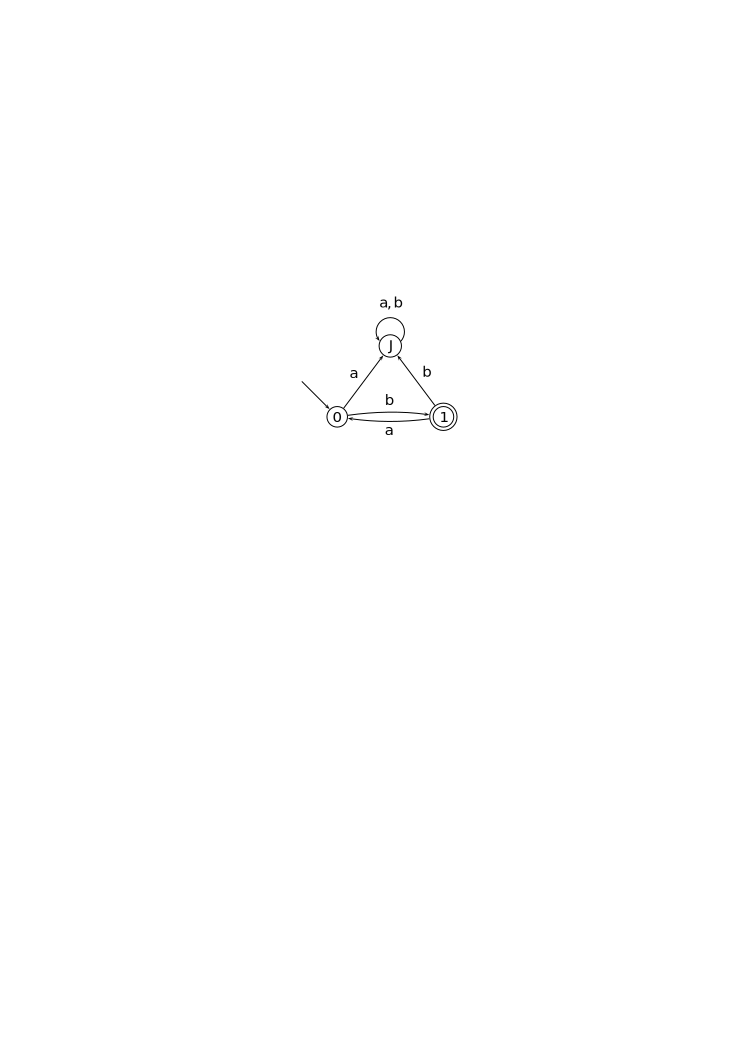
\includegraphics[width=0.7\linewidth]{automaten/Loesung2.pdf}
	\end{figure}
\end{frame}

% TODO: Fix dirty hack in thwregex.sty, where I changed line 42 to print star in math-mode
% 		because otherwise the star was always raised in my config.
%	COmment(Daniel): Reverted your change. No problems whatsoever.
%		Use \rx everywhere

% Fuck you, Latex. In my algo tutorial slides, this isn't necessary. Why here then!?
\begin{frame}[t]
	\fakeframetitle{\only<2->{Grenzen endlicher Akzeptoren}}
	Gibt es einen endlichen Akzeptor $A$ mit $$L(A) = \set{ \word a^k\word b^k \Mid k\in \N_0 }?$$
	\pause
	Nein! Warum nicht? \visible<3->{Endliche Automaten können nicht unendlich weit „zählen“!}\\
	
	Gibt es einen endlichen Akzeptor, der alle gültigen Klammerausdrücke erkennt?\\ \pause
	Nein, aus dem selben Grund.
	\begin{figure}[H]
		\includegraphics[scale=0.5]{xkcd/tags_1144}
		\caption{ \texttt{\url{https://www.xkcd.com/1144/}} }
	\end{figure}
	\pause
	Kontextfreie Grammatiken \enquote{können also mehr} als endliche Akzeptoren.\\
	Wir wollen nun ein \enquote{gleichmächtiges} Konzept zu Akzeptoren.
\end{frame}

\section{Reguläre Ausdrücke}
\subsection{Definition}

\begin{frame}{Disclaimer!}
	\begin{center}
		\Large
			\bfalert{\Huge ACHTUNG!} \\ \medskip
		
		Gemeint sind \textbf{NICHT} sog. \emph{Regular Expressions}, die ihr vllt. aus Programmiersprachen kennt! \\ \bigskip
		
		{\normalsize (Die sind ähnlich, aber eben nicht das gleiche.)}
	\end{center}
\end{frame}

\begin{frame}{Reguläre Ausdrücke}
	Wir können uns reguläre Ausdrücke zusammenbauen aus
	\begin{itemize}
		\item den einzelnen Symbolen $x$ aus $A$ \pause
		\item zwei regulären Ausdrücken $R_1$ und $R_2$ mit $$\rx(R_1 R_2\rx) \qquad \text{ oder } \qquad \rx(R_1\rx|R_2\rx)$$ \pause
		\item einem Stern $R\rx*$ \pause
		\item oder dem leeren Ausdruck $\rx O$ \pause
	\end{itemize} 
	Klammern dürfen nach den Klammerregeln weggelassen werden:\\
	Stern vor „Punkt“ {\small (in diesem Fall unsichtbar)} vor Strich.
\end{frame}

\begin{frame}{Reguläre Ausdrücke}
	\begin{Beispiel}
		Sei $ A = \{ \word a, \word b, \word c\}$. Dann sind gültige reguläre Ausdrücke über $A$:\\
		$\rx{abc}$\\
		$\rx{a|b|c}$\\
		$\rx{(ab)*}$\\
		$\rx{O*}$
	\end{Beispiel}
\end{frame}


\begin{frame}{Sprache eines Ausdruckes}
	Die durch $R$ beschriebene Sprache $\lang{R}$ ist wie folgt definiert:
	\begin{itemize}
		\item $\lang{\rx{O}} = \emptyset$
		\item $\lang{x}=\{x\} \quad (\text{für }x\in A)$
		\item $\lang{R_1 \rx| R_2} = \lang{R_1} \cup \lang{R_2}$
		\item $\lang{R_1 R_2} = \lang{R_1} \cdot \lang{R_2}$
		\item $\lang{R\rx*} = \lang{R}^*$
	\end{itemize} 

	\bigskip
	Eine Sprache, für die es einen beschreibenden regulären Ausdruck gibt, nennt man \textbf{regulär}.
\end{frame}

\begin{frame}{Sprache eines Ausdruckes}
	\begin{Beispiel}
		\begin{itemize}
			\item $\lang{\rx{a}} = \{\word a\}$. \pause
			\item $\lang{\rx{ab}} = \lang{\rx{a}} \cdot \lang{\rx{b}} = \{\word a\word b\}$. \pause
			\item $\lang{\rx{a|b}} = \lang{\rx{a}}\cup\lang{\rx{b}} = \{\word a,\word b\}$. \pause
			\item $\lang{\rx{(a|b)*}} = \lang{\rx{a|b}}^* = \{\word a,\word b\}^*$. \pause
			\item $\lang{\rx{(a*b*)*}} = \lang{\rx{a*b*}}^* = \left(\lang{\rx{a*}}\lang{\rx{b*}}\right)^* 
			= \left(\lang{\word a}^*\lang{\word b}^*\right)^* = \left(\{\word a\}^* \· \{\word b\}^*\right)^*$\\
			$= \{\word a,\word b\}^*$.  
		\end{itemize}
	\end{Beispiel}
	\pause
	\begin{block}{Aufgabe}
		Gebt einen regulären Ausdruck $R$ an mit $\lang{R} = $  
		\begin{itemize}
			\item die Sprache aller binären Zweierpotenzen \\ \visible<+->{}
				  \visible<+-|handout:2>{\impl $R = \rx{0*10*}$}
			\item die Sprache aller geraden Binärzahlen \\
				  \visible<+-|handout:2>{\impl $R = \rx{(0|1)*0}$}
		\end{itemize}
	\end{block}
\end{frame}

\begin{frame}{Aufgabe: Reguläre Ausdrücke}
	In dieser Aufgabe geht es um die formalen Sprachen
	$$L_1 = \set{\word a^k \word b^m \Mid k, m \in \N_0 }, \qquad L_2 = \set{\word b^k \word a^m \Mid k, m \in \N_0 }.$$
	Gebt für jede der folgenden formalen Sprachen $L$ je einen regulären Ausdruck $R$ an mit $ \langle R \rangle = L$.
	\begin{itemize}
		\item $L = L_1 \cup L_2$ \\
			\visible<2-|handout:2>{$ \rx{a*b*|b*a*}$}
		\item $L = L_1 \cap L_2$ \\
			\visible<3-|handout:2>{$ \rx{a*|b*}$}
		\item $L = L_1\cdot L_2$ \\
			\visible<4-|handout:2>{$ \rx{a*b*b*a*}$ oder $\rx{a*b*a*}$}
		\item $L = L_1^*$ \\
			\visible<5-|handout:2>{$ \rx{(a*b*)*}$ oder $\rx{(a|b)*}$}
	\end{itemize}
\end{frame}

\begin{frame}{Aufgabe: Sprachen regulärer Ausdrücke}
	\begin{itemize}
		\item $\lang{\rx{(a|b)*abb(a|b)*}} = \visible<2-|handout:2>{\{\word a, \word b\}^* \cdot \{\word a\word b\word b\} \cdot \{\word a, \word b\}^*}$
		\item $\lang{\rx{a**}} = \visible<3-|handout:2>{\{\word a\}^*}$
		\item $\lang{\visible<4-|handout:2>{R\rx{(}R\rx{)*}}} = \lang{R}^+$ \quad (für bel. reg. Ausdruck $R$)
		\item $\lang{\visible<5-|handout:2>{\rx{O*}}} = \{\eps\}$
		\item $\lang{\visible<6-|handout:2>{\rx{a*ba*ba*b(a|b)*}}} = \set{ w \in \{\word a, \word b\}^* \Mid \size{w}_{\word b} > 2 } $
		\item $\lang{\visible<7-|handout:2>{\rx{b*a*}}} =$ Sprache aller Wörter über $\set{\word a, \word b}$, in denen das Teilwort \word{ab} nicht vorkommt.
	\end{itemize}
\end{frame}



\section{Strukturelle Induktion}
\subsection{Kantorowitsch-Bäume}
\begin{frame}
	Man kann syntaktische Ausdrücke als Kantorowitsch-Baum schreiben. \\
	Beispiel: einfacher arithmetischer Ausdruck: $3 + (a + b) \cdot (-c)$ \pause
	\begin{figure}[H]
		\centering
		\includegraphics[width=0.4\linewidth]{struktInd/Baum.pdf}
	\end{figure}
\end{frame}

\subsection{Strukturelle Induktion}
\begin{frame}
	Aussagen mit z.B. regulären Ausdrücken, Produktionsmengen o.Ä. lassen sich am Besten über \textbf{strukturelle Induktion beweisen} \pause
	Dabei zeigt man:
	\begin{description}[<+->]
		\item[Induktionsanfang] Die Aussage stimmt für die Wurzel / jedes Atom
		\item[Induktionsvoraussetzung] Die Aussage stimmt für einen Teilbaum / einen Teilausdruck
		\item[Induktionsschluss] Die Aussage stimmt für jede Verzweigung / jeden Produktionsschritt
	\end{description}
\end{frame}

% TODO: Austauschen gegen nicht-Klausuraufgabe (Klausur März 2011)
\begin{frame}{Aufgabe}
	Die Menge $M \subset \N_0$ sei definiert durch:
	\begin{itemize}
		\item 5 und 8 liegen in $M$.
		\item Für alle $m$, $n$ gilt: Wenn $n$ und $m$ in $M$ liegen, dann ist auch $n^2 + m^2$ in $M$.
		\item Keine anderen Zahlen liegen in $M$.
	\end{itemize}
	Zeigen Sie durch strukturelle Induktion:
		$$\forall \ n \in M : n \mod 3 = 2$$
\end{frame}

\begin{frame}{Lösung}
	\begin{description}[<+->]
		\item[Induktionsanfang] $5 \mod 3 = 8 \mod 3 = 2$
		\item[Induktionsvoraussetzung]
Für beliebige aber feste $n, m \in M$ gelte: $$n \mod 3 = 2 \text{ und } m \mod 3 = 2$$
		\item[Induktionsschritt:] Wir zeigen, dass dann auch $(n^2 + m^2 ) \mod 3 = 2$ gilt. \pause \\
		Aus $n \mod 3 = 2$ folgt $$n^2 \mod 3 = (n \mod 3)^2 \mod 3 = 2^2 \mod 3 = 4 \mod 3 = 1$$ Ebenso gilt $m^2 \mod 3 = 1$, und es folgt $$(n^2 + m^2 ) \mod 3 = 1 + 1 = 2$$
	\end{description}
\end{frame}


\begin{frame}	
	\begin{block}{Was ihr nun wissen solltet}
		\begin{itemize}
			\item Reguläre Ausdrücke
			\item Rechtslineare Grammatiken
		\end{itemize}
	\end{block}
	
	\begin{block}{Was nächstes Mal kommt}
		\begin{itemize}
			\item Turingmaschinen - Mächtiger wird es nicht mehr!
		\end{itemize}
	\end{block}
\end{frame}

\xkcdframe{0.5}{30}{xkcd/houston_1438.png}{http://www.xkcd.com/1438}{Oh, hi mom. No, nothing important, just work.}

\slideThanks

\end{document}